\documentclass[a4paper,12pt]{article}

% Pacotes necessários
\usepackage[utf8]{inputenc}
\usepackage[brazil]{babel}
\usepackage{hyperref}
\usepackage[T1]{fontenc}
\usepackage{graphicx}
\usepackage{caption}
\usepackage[left=2cm, right=2cm, top=2cm, bottom=2cm]{geometry}
\usepackage{lipsum} % Para gerar texto de preenchimento
\usepackage{float}
\usepackage{amsmath}
\usepackage{listings}
\usepackage{xcolor}


% Configuração da página de título
\newcommand{\reporttitle}{Trabalho 2 - Reator}
\newcommand{\reportauthor}{
Lucas William Junges}
\newcommand{\reportdate}{30/06/2025}
%\renewcommand{\listoffigures}{}
%\renewcommand{\tableofcontents}{}


\begin{document}

% Página de título personalizada
\begin{titlepage}
    \centering
    \vspace*{1cm}
    
\includegraphics[width=0.4\textwidth]{Imagens/BrasaoUFSC.png} % Adicione o caminho para o logotipo da sua instituição
    \par\vspace{1cm}
    {\scshape\Large Universidade Federal de Santa Catarina\par} % Substitua pelo nome da sua instituição
    \vspace{1.2cm}
    {\huge\bfseries \reporttitle\par}
    \vspace{2cm}
    {\Large\itshape \reportauthor\par}
    \vfill
    {\large \reportdate\par}
\end{titlepage}

% Lista de ilustrações
\listoffigures
\clearpage

% Sumário
\tableofcontents
\clearpage



\section{Introdução}

Na primeira parte deste trabalho, foi realizada uma análise detalhada e o desenvolvimento inicial de um sistema de controle de concentração de produto em um reator continuamente agitado, amplamente utilizado na indústria química. Este sistema visa a produção de cyclopentenol (produto B) a partir de cyclopentadiene (produto A), com a presença de um catalisador diluído em água, além de produzir subprodutos como dicyclopentadiene (produto D) e cyclopentanediol (produto C).

A dinâmica do processo foi modelada considerando parâmetros constantes do reator e utilizando a variável manipulada \(u = \frac{F}{V}\) e a concentração de entrada \(C_{AF}\) como perturbação principal. A análise incluiu a determinação de um ponto de operação específico e a linearização do modelo não linear ao redor desse ponto, facilitando o desenvolvimento do controle.

Nesta segunda parte do trabalho, o foco será o desenvolvimento e a implementação de técnicas avançadas de controle para melhorar o desempenho do sistema de reator. Será projetado um controle contínuo utilizando a técnica de lugar de raízes, visando atender a especificações rigorosas de desempenho, como tempo de acomodação e pico máximo de resposta. Este novo controlador será comparado ao controlador PI desenvolvido na primeira parte, utilizando simulações para avaliar sua eficácia.

Além disso, será simulado o comportamento dinâmico do sistema completo e não linear para verificar a robustez do controle implementado. Esta simulação incluirá cenários realistas de operação, como variações e perturbações próximas ao ponto de operação, permitindo uma análise detalhada do desempenho do controlador.

Será explorada a possibilidade de aprimorar o controle do sistema através da inclusão de um sensor adicional de concentração. Dois sistemas de controle serão propostos, um utilizando a medição de \(C_{AF}\) e outro a medição de \(C_A\), e suas performances serão comparadas para determinar a solução mais eficiente. A implementação final do controle escolhido será realizada em Matlab, considerando a discretização adequada para garantir a precisão do controle digital.

Por fim, será feita uma simulação abrangente do sistema não linear com o controle proposto, incluindo variações de referência e perturbações, além da simulação de ruídos de medição para criar um cenário mais realista. Os resultados serão comparados com os obtidos na primeira parte do trabalho, proporcionando uma visão completa sobre a eficácia das diferentes abordagens de controle.

O objetivo desta pesquisa é aprofundar o conhecimento sobre os princípios de controle e análise de sistemas dinâmicos aplicados a processos químicos industriais, utilizando tanto ferramentas teóricas quanto de simulação para projetar e avaliar estratégias de controle eficazes.

\newpage

% Desenvolvimento
\section{Desenvolvimento}
\label{chap:desenvolvimento}

Na Parte 1, foi analisado o modelo e o sistema de controle de concentração de produto em um reator continuamente agitado, usado na indústria química. O controle utilizado foi um PI básico de \(C_B\), ajustado por alocação de polos.

A dinâmica de produção dos produtos A e B foi modelada nas proximidades de um ponto de operação, definido por \(C_{AF} = 5.1\) mol/L e \(u = 0.8\) 1/min. O reator possui os seguintes parâmetros: \(k_1 = 6.01\) 1/min, \(k_2 = 0.8433\) 1/min, e \(k_3 = 0.1123\) mol/(L min). Lembrando que o sistema utiliza \(u = \frac{F}{V}\) como variável manipulada e \(C_{AF}\) (concentração da entrada) como perturbação. A variável \(u\) pode variar entre 0 e 10 L/min, e a concentração de entrada \(C_{AF}\) entre 4.0 e 6 mol/L.

O modelo a ser utilizado no projeto do controle foi obtido pela linearização analítica do modelo não linear nesse ponto de operação. Este novo modelo também considera a dinâmica de \(C_A\). Assim, pode-se escrever:

\begin{equation}
(s + 1.6433) C_B(s) = 6.01 C_A(s) - 2.1699 U(s)
\end{equation}

\begin{equation}
(s + 6.9433) C_A(s) = 0.8 C_{AF}(s) + 4.5067 U(s)
\end{equation}

Recomenda-se desenhar um diagrama de blocos deste modelo para visualizar a relação entre as variáveis.

 \begin{figure}[ht]
  \centering
  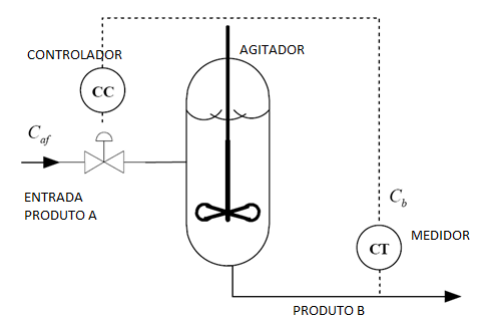
\includegraphics[width=0.6\textwidth]{Imagens/Reator.png}
 % \caption{Reator}
  \end{figure}

\newpage

\section{Parte 2 -  Análise e Projeto por Lugar das Raízes}
\subsection{Projeto de Controle por Lugar das Raízes}

a) Projete um controle contínuo usando a técnica de lugar de raízes para obter em malha fechada um sistema com \(t_{5\%}\) da ordem de 1.5 minutos e pico menor que 5\%. Essa especificação deve ser atendida para resposta a seguimentos de degraus de referência de \(C_B\) e perturbações de \(C_{AF}\). Use filtro de referência se necessário. O sistema deve ter ganho estático unitário para a relação referência-saída de \(C_B\).\\


Como na parte 1 do trabalho foram encontradas as funções de transferência da concentração \(C_B\) em função da concentração \(C_A\) e entrada \(U\) e também a função de transferência da concentração \(C_A\) em função de \(C_{AF}\) e entrada \(U\), deduz-se:

\begin{align}
\Delta C_a(s) &= \frac{\Delta C_{af}(s) + 4.381 \Delta u(s)}{s + 7.171} = \frac{\Delta C_{af}(s)}{s + 7.171} + \frac{4.381 \Delta u(s)}{s + 7.171}
\end{align}
\begin{align}
\Delta C_b(s) &= \frac{6.01 \Delta C_a(s) - 2.354 \Delta u(s)}{s + 1.843} = \frac{6.01 \Delta C_a(s)}{s + 1.843} - \frac{2.354 \Delta u(s)}{s + 1.843}
\end{align}

Substituindo a equação (3) na equação (4), tem-se:

\begin{align}
\Delta C_b(s) &= \frac{6.01}{s + 1.843}\left(\frac{\Delta C_{af}(s)}{s + 7.171} + \frac{4.381 \Delta u(s)}{s + 7.171}\right) - \frac{2.354 \Delta u(s)}{s + 1.843}\\
\Delta C_b(s) &= \frac{6.01\Delta C_{af}}{(s + 1.843)(s + 7.171)} + \frac{26.329\Delta u(s)}{(s + 1.843)(s + 7.171)} - \frac{2.354 \Delta u(s)}{s + 1.843}\\
\Delta C_b(s) &= \frac{6.01}{(s + 1.843)(s + 7.171)}\Delta C_{af} - \frac{2.354(s-4.013)}{(s + 1.843)(s + 7.171)}\Delta u(s)\\
\end{align}

Dessa forma, as duas funções de transferência que relacionam a concentração \(C_B\) com a concentração \(C_AF\) e a entrada \(U\) são:

\begin{align}
\frac{ C_b(s)}{C_{af}} = \frac{6.01}{(s + 1.843)(s + 7.171)}\\
\frac{ C_b(s)}{u(s)} = \frac{-2.354(s-4.013)}{(s + 1.843)(s + 7.171)}
\\
\end{align}


Como os parâmetros exigidos de projeto de controle especificam que o tempo de assentamento é de 1.5 minutos e pico máximo permitido é 5\%, o fator de amortecimento pode ser definido por:

\begin{align}
\xi = \sqrt{\frac{1}{(\frac{\pi}{ln(0.005})^2+1}} = 0.69\\
\omega_n = \frac{3}{\xi*t_{5\%}} = \frac{3}{0.86*1.5} = 2.8986
\end{align}

A partir disso, o polo desejado  para atender os parâmetros de operação exigidos é: 

\begin{align}
P_d = - \xi*\omega_n \pm \omega_n*\sqrt{1-j\xi^2}\\
P_d = - 0.69*2.8986 \pm 2.8986 \sqrt{1-j0.4761}\\
P_d = -2 \pm j2.0976
\end{align}

Ao analisar a função de transferência (10) e assumindo que o controlador incorpora o modo característico de rejeição de entradas do tipo degrau para atender às condições especificada. Tem-se que o ganho do lugar das raízes:
\begin{align}
K_{LR} = -2.354*K_c    
\end{align}

Então:

\begin{alignat}{3}
K_E &> 0, & \quad K_C &> 0, & \quad k_{LR} &< 0
\end{alignat}

Ou seja, desta forma, considerando que:
\[ C(s) = K_c \cdot \frac{N_c}{D_c'} \leftrightarrow (6.7) \]

Tem-se:

\begin{align}
\theta_1 = 180^\circ - \tan^{-1} \left( \frac{2.0976}{|-2 - 4.013|} \right) = 160.0547^\circ\\
\theta_2 = 180^\circ - \tan^{-1} \left( \frac{2.0976}{|-2 - 0|} \right) = 133.4567^\circ\\
\theta_3 = 180^\circ - \tan^{-1} \left( \frac{2.0976}{|-2 + 1.843|} \right) = 93.1026^\circ\\
\theta_4 = 180^\circ - \tan^{-1} \left( \frac{2.0976}{|-2 + 7.171|} \right) = 21.1495^\circ\\ 
\phi_{NC} - \phi_{Dc'} + \theta_1 - \theta_2 - \theta_3 - \theta_4 = 0^\circ\\
\phi_{NC} - \phi_{Dc'} = 87.6541^\circ
\end{align}

Considerando a fase positiva, é necessário adicionar zeros ao controlador. No entanto, adicionar apenas um zero com uma fase de 87.6541° praticamente eliminaria o efeito do polo desejado. Para resolver isso, optamos por incluir dois zeros, cada um com metade da fase resultante, além de um polo adicional, tornando o controlador matematicamente próprio.

\begin{align}
C(s) = \frac{K_C(s + z_1)(s + z_2)}{s(s + p)}
\end{align}

Como prática consistente em projeto de controladores, adiciona-se um polo extra dez vezes mais rápido que a parte real do polo complexo conjugado desejado:

\begin{align}
p = 10*(-2) = -20
\end{align}

E portanto, uma fase adicional $\theta_5$:

\begin{align}
\theta_5 = \arctan(\frac{2.0976-0 }{-2+20})  = 6.6304^\circ
\end{align}
 Refazendo o somatório considerando a nova fase:
 
 \begin{align}
 \phi_{NC}-\phi_{DC}-\theta_5=87.6541^\circ\\
 \phi_{NC}-\phi_{DC}=94.2845^\circ
 \end{align}

 Então, as fases dos zeros devem ser metade disso, $47.1423^\circ$ e, portanto:

 \begin{align}
     |tan(47.1423)|=\frac{2.0976}{-2-z}\\
     z = -3.835
 \end{align}

 O ganho do lugar das raízes é definido a partir da relação:

 \begin{align}
|K_{LR}|= \left|\frac{A(s)}{B(s)}\right|_{s\rightarrow pd}\\
K_{LR} = \left|\frac{s(s+1.843)(s+7.171)(s+20)}{(s+3.835)^2*(s+4.013)}  \right|_{s\rightarrow pd} = 12.4635
 \end{align}

 Substituindo o valor do ganho do lugar das raízes encontrado em (17), o ganho do controlador é:

 \begin{align}
     K_c = \left|\frac{K_LR}{2.354}  \right|= 5.2946
 \end{align}

 Assim, o controlador será definido por:
\begin{align}
  C(s)=\frac{5.2946(s+3.835)^2}{s(s+20)}  
\end{align}

Pela disposição de dois zeros dominantes em -3.835 e dois polos em 0 e -20, se faz necessário a utilização de um filtro de referência, garantindo a estabilidade:

\begin{align}
    F_r=\left (\frac{z}{s+z}\right)^2 = \left (\frac{3.835}{s+3.835}\right)^2
\end{align}
 
b) Estude o comportamento do sistema sobre o modelo linearizado por simulação.
Realize análise dos diagramas polo-zero e da resposta em frequência do sistema e 
interprete os resultados. Observe o sinal de controle nos ensaios realizados. 
Compare este controle com o PI projetado na parte 1. Discuta.

\begin{figure}[H]
    \centering % Centraliza a imagem
    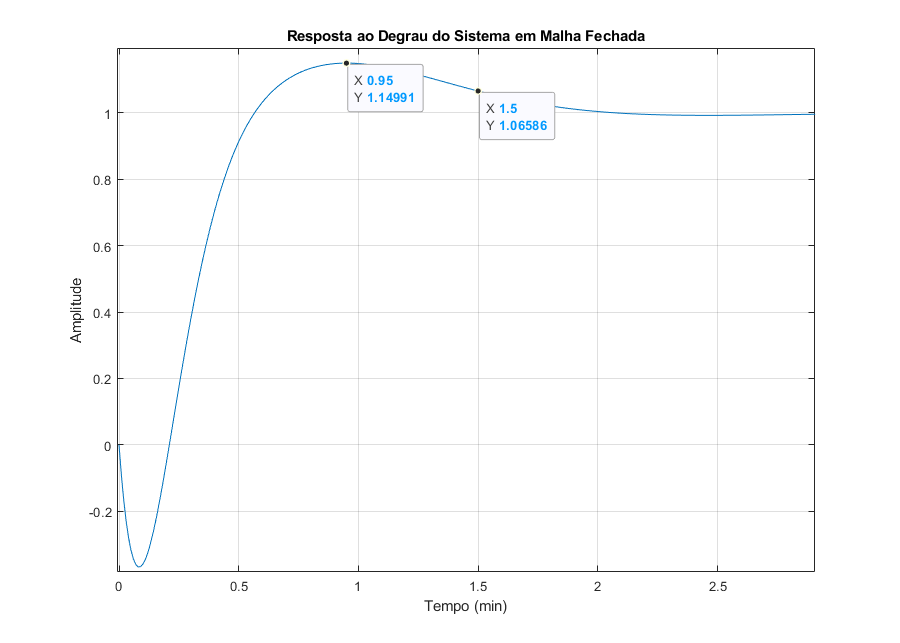
\includegraphics[width=0.8\textwidth]{Imagens/1B/1BRespostaMFDegrauAutoral2.png} % Inclui a imagem
    \caption{Resposta ao Degrau de Y/R}
    \label{fig:exemplo} % Adiciona um rótulo para referenciar a imagem no texto
\end{figure}

A resposta ao degrau fornece a dinâmica do sistema em tempo, mostrando como ele reage a uma entrada de degrau unitário. O sistema apresenta uma resposta rápida e um overshoot controlado, indicando uma boa estabilidade e desempenho. O erro em regime permanente próximo de zero indica precisão no rastreamento de referência.

\begin{figure}[H]
    \centering % Centraliza a imagem
    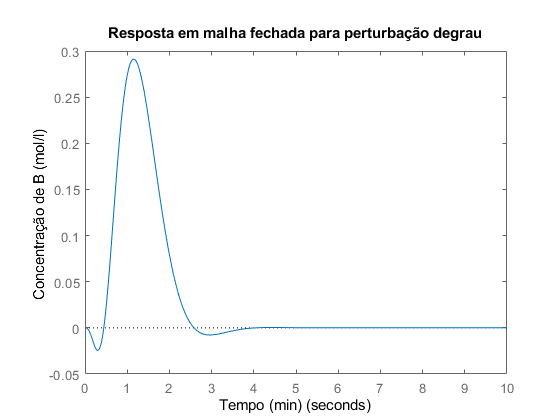
\includegraphics[width=0.8\textwidth]{Imagens/1B/1BRespostaPerturbaçãoAutoral.png} % Inclui a imagem
    \caption{Resposta ao Degrau de Y/Q}
    \label{fig:exemplo} % Adiciona um rótulo para referenciar a imagem no texto
\end{figure}

A resposta ao degrau de Y/Q demonstra como o sistema reage a uma mudança abrupta em Q, que pode ser interpretada como uma perturbação. A resposta rápida com um overshoot controlado indica que o sistema retorna rapidamente ao estado de equilíbrio após uma perturbação. O pequeno ou nulo erro em regime permanente demonstra que o sistema é capaz de rejeitar a perturbação e manter o desempenho desejado.
 

\begin{figure}[H]
    \centering % Centraliza a imagem
    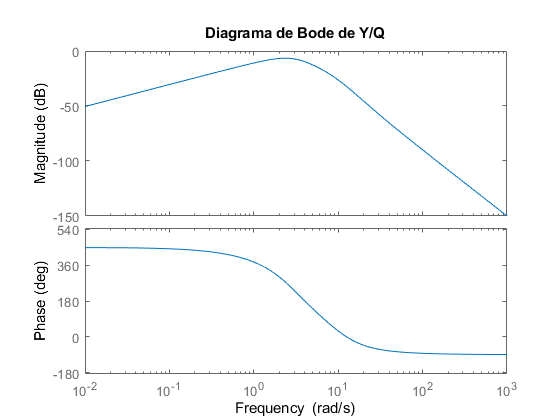
\includegraphics[width=0.8\textwidth]{Imagens/1B/1BbodeYQAutoral.png} % Inclui a imagem
    \caption{Diagrama de Bode de Y/Q}   
\end{figure}

O diagrama de Bode para Y/Q mostra a resposta em frequência desta função de transferência específica. Uma margem de fase e ganho adequadas confirmam a estabilidade e a robustez do sistema sob perturbações específicas. Um detalhe para atenuação de entradas de baixíssimas frequências.

\begin{figure}[H]
    \centering % Centraliza a imagem
    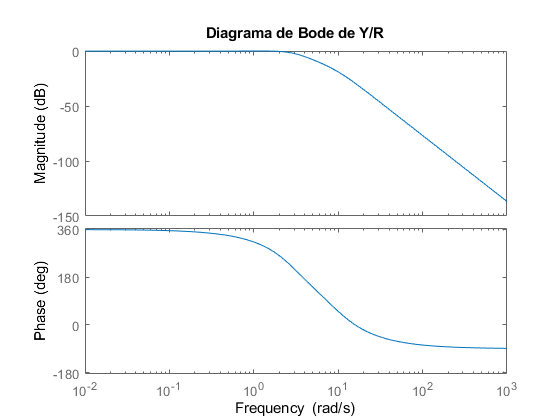
\includegraphics[width=0.8\textwidth]{Imagens/1B/1BbodeYRAutoral.png} % Inclui a imagem
    \caption{Diagrama de Bode de Y/R}
\end{figure}

O diagrama de Bode de Y/R mostra a resposta em frequência do sistema, fornecendo informações sobre o ganho e a fase em função da frequência. O ganho indica a amplificação ou atenuação do sinal em diferentes frequências, enquanto a fase mostra o atraso introduzido pelo sistema em várias frequências. Uma margem de fase positiva e uma margem de ganho adequada indicam que o sistema é estável e pode resistir a pequenas perturbações.

\begin{figure}[H]
    \centering % Centraliza a imagem
    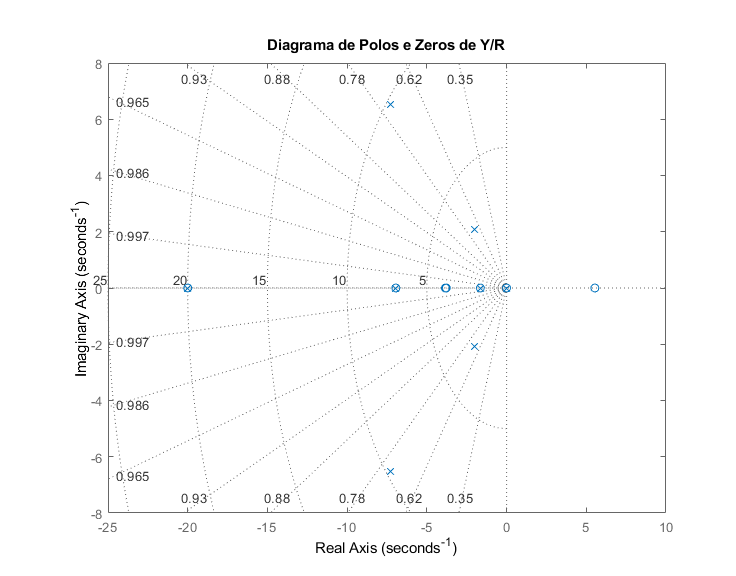
\includegraphics[width=0.8\textwidth]{Imagens/1B/1BDiagramaYRpolozeroAutoral.png} % Inclui a imagem
    \caption{Diagrama Polo e Zero Y/R}
\end{figure}

O diagrama polo-zero para Y/R nos mostra a distribuição dos polos e zeros da função de transferência Y/R. Os polos estão associados aos modos naturais do sistema, enquanto os zeros indicam frequências que atenuam a resposta. Os polos permanecem no semiplano esquerdo, indicando estabilidade assintótica dessa função. A presença de zero no semiplano direito sugere o aparecimento de reposta de fase não mínima.

\begin{figure}[H]
    \centering % Centraliza a imagem
    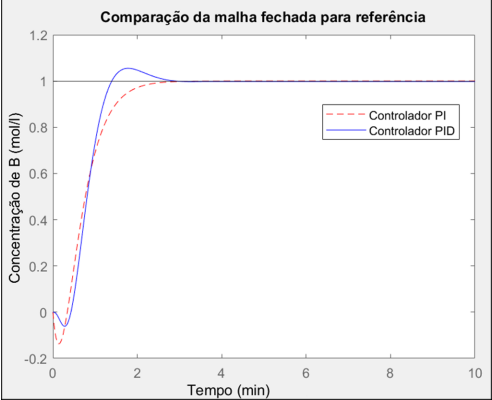
\includegraphics[width=0.7\textwidth]{Imagens/1B/1BComparacaoPILR.png} % Inclui a imagem
    \caption{Comparaçao PI e PID-LR}
\end{figure}

A análise e comparação entre os controladores PI e PID para um sistema de controle revelam diferenças significativas em termos de desempenho, estabilidade e capacidade de resposta a perturbações. Cada um desses controladores é projetado com base em modelos matemáticos que aproximam o comportamento dinâmico do sistema real, mas suas abordagens e resultados variam consideravelmente dependendo da complexidade da planta.

O controlador PI é amplamente utilizado devido à sua simplicidade e eficácia na eliminação do erro em regime permanente. No entanto, sua aplicação é mais adequada para sistemas que podem ser adequadamente modelados por funções de transferência de primeira ordem. Em sistemas mais complexos, como os de segunda ordem, o PI pode introduzir oscilações não desejadas e uma resposta de fase que não minimiza de forma eficiente. Isso ocorre porque a dinâmica do PI não é idealmente compatível com a dinâmica mais complexa do sistema. A capacidade do PI em rejeitar perturbações é limitada em comparação com o PID. Ele pode resultar em maiores overshoots e tempos de acomodação prolongados quando o sistema é sujeito a mudanças bruscas ou perturbações externas.

Por outro lado, o controlador PID oferece uma abordagem mais sofisticada e adaptável para sistemas de controle mais complexos, especialmente aqueles que exibem dinâmicas de segunda ordem. Ele é capaz de ajustar suas constantes proporcionais, integrais e derivativas para otimizar a resposta do sistema de acordo com as necessidades dinâmicas específicas. O PID é mais eficaz na minimização de oscilações e na obtenção de uma resposta de fase mínima, o que resulta em um controle mais preciso e estável do sistema. Devido à sua capacidade de ajuste fino e resposta rápida, o PID demonstra uma melhor capacidade de rejeitar perturbações. Isso garante que o sistema retorne rapidamente ao estado desejado após ser perturbado, mantendo a estabilidade operacional.

Enquanto o controlador PI é adequado para sistemas simples de primeira ordem, ele se mostra limitado quando aplicado a sistemas mais complexos, como os de segunda ordem. O controlador PID, com sua capacidade de modelagem mais refinada e ajuste dinâmico, oferece uma solução mais robusta e eficiente para esses casos. Sua capacidade de proporcionar uma resposta rápida, estável e precisa faz com que seja a escolha preferencial em muitas aplicações industriais e de controle avançado.

\newpage









\subsection{Simulação}

a) Usando Simulink, estude por simulação o comportamento dinâmico do sistema em MF 
com o modelo completo não linear e verifique se atende as especificações. 
Implemente um cenário de simulação com a partida do sistema em rampa até chegar 
no ponto e operação. Simule, então, variações perto do ponto de operação e aplique 
perturbações. Que acontece com o sistema ao se afastar do ponto de operação?
Compare este controle com o PI projetado e discuta

Usando U=0.8 e Caf = 5.1, como dado no enunciado, temos que o valor final é de:

Estudando o comportamento do sistema com os valores de entrada, obtemos o ponto
de operação do sistema.

\begin{figure}[H]
    \centering
    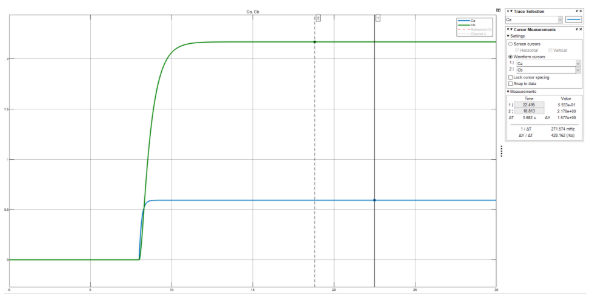
\includegraphics[width=0.8\linewidth]{image7.png}
    \caption{Ponto de operação do sistema}
    
\end{figure}

\begin{align}
C_b = 2.17 mol/l
C_a = 0.5933 mol /l
\end{align}


Desenvolvendo a simulação do sistema não linear com a implementação do sistema de controle projetado, obtemos o seguinte diagrama do Simulink.

\begin{figure}[H]
    \centering
    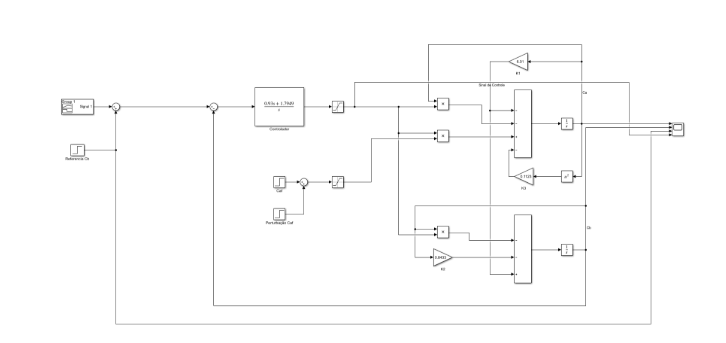
\includegraphics[width=0.8\linewidth]{image8.png}
    \caption{Diagrama de blocos do sistema não linear}
    
\end{figure}

O gerador de sinais utiliza uma rampa para levar o sistema ao ponto de operação, e então o sinal tipo rampa é desligado. O tempo necessário para levar o sistema ao ponto de operação foi de 8 segundos, após este tempo, o sinal de referência é ligado e então o sistema de controle passa a atuar mantendo o sistema no ponto de operação.

\begin{figure}[H]
    \centering
    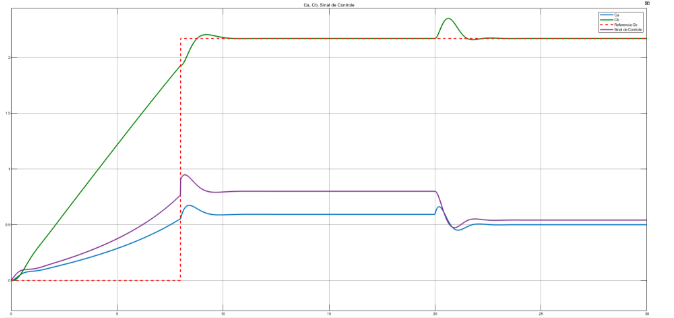
\includegraphics[width=0.8\linewidth]{image9.png}
    \caption{Resposta do sistema no Ponto de operação}
    
\end{figure}

Afastando a referência do sistema do ponto de operação, (Ref = 2,60) obtemos:

\begin{figure}[H]
    \centering
    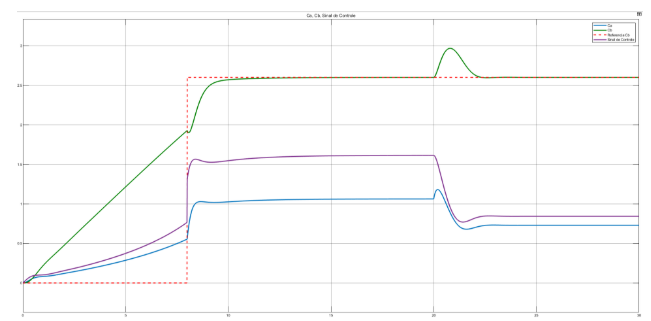
\includegraphics[width=0.8\linewidth]{image10.png}
    \caption{Resposta do sistema com Ref = 2,60}
    
\end{figure}

Afastando mais o ponto de operação (Ref = 2,80), o sistema de controle não consegue estabilizar o sistema.

\begin{figure}[H]
    \centering
    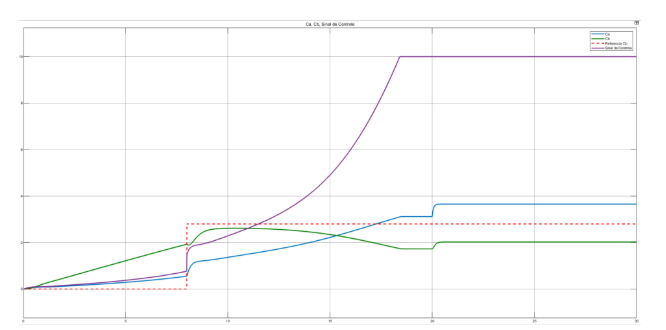
\includegraphics[width=0.8\linewidth]{image11.png}
    \caption{ Resposta do sistema com Ref = 2,80}
    
\end{figure}

O sistema em malha fechada não consegue se manter estável pois o controlador foi projetado baseando-se numa aproximação linear do sistema não linear, próximo ao ponto de operação, os dois modelos se comportam de maneira muito semelhante próximos ao ponto
de operação. Ao se afastar do ponto de operação, os modelos divergem e o sinal de controle enviado não é o correto. 

Comparando com o projeto por PI realizado na questão anterior, pudemos perceber que este controlador parece ser um pouco mais robusto, conseguindo manter o sistema estável com uma variação maior do ponto de operação. Outro ponto é referente as oscilações, o controlador PI faz com que o sistema tenha oscilações antes de estabilizar, enquanto que este não oscila.

\newpage
\subsection{Sobresensoriameno}

Considere agora que dispõe de mais um sensor de concentração que pode ser usado 
para medir CAF ou CA.

a) Proponha dois sistemas de controle, um com cada uma das medições disponíveis, 
de forma a melhorar o desempenho obtido no item 2. Ajuste estes dois novos 
sistemas de controle, compare e decida qual é mais interessante. Pode realizar os 
projetos no plano s. Usando ainda o processo modelado de forma linear simule, 
analise diagramas polo-zero e interprete os resultados.

Para o controle Feed-Forward de \(C_{af}\), podemos realizar os seguintes cálculos:

\begin{align}
G_{q1} &= \frac{C_b}{C_{af}} = \frac{4.81}{(s + 6.94)(s + 1.64)}, \\
G &= \frac{C_b}{U} = \frac{-2.17(s-5.54)}{(s + 6.94)(s + 1.64)}.
\end{align}

E temos que:

\begin{align}
C_{ff1} = \frac{G_{q1}}{G}
\end{align}

Dessa forma:

\begin{align}
C_{ff1} = \frac{\frac{4.81}{(s+6.94)(s+1.64)}}{\frac{-2.17(s-5.54)}{(s+6.94)(s+1.64)}} = \frac{4.81}{-2.17(s-5.54)}
\end{align}

Como \(C_{ff1}\) é instável, vamos propor 2 alternativas. A primeira é trocar o polo instável que está no semiplano direito para um polo no semiplano esquerdo e ajustar o ganho.

\begin{align}
C_{ff1} = \frac{2.217}{(s+5.54)} \approx -0.4
\end{align}

Utilizando a seguinte estrutura de controle:

\begin{align}
C_{ff1} = \frac{-2.217}{(s+5.54)}
\end{align}
Construímos a seguinte estrutura de controle para o sistema linear:

\begin{figure} [H]
    \centering
    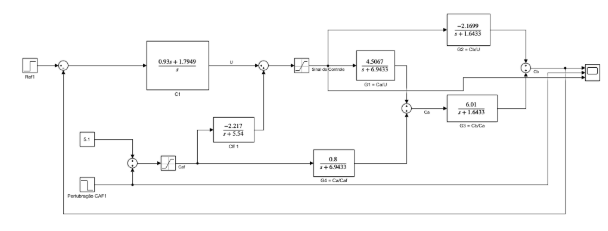
\includegraphics[width=0.8\linewidth]{image12.png}
    \caption{Diagrama de Blocos do sistema linear com Cff1}    
\end{figure}

Obtemos a seguinte resposta em malha fechada no sistema linear: 

\begin{figure} [H]
    \centering
    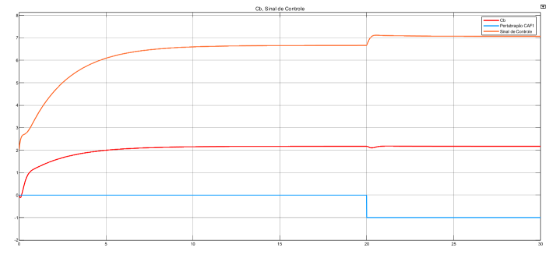
\includegraphics[width=0.8\linewidth]{image13.png}
    \caption{Resposta do sistema linear}    
\end{figure}

Trocando agora a estrutura de controle:

\(C_{ff1}\) = - 0.4

\begin{figure} [H]
    \centering
    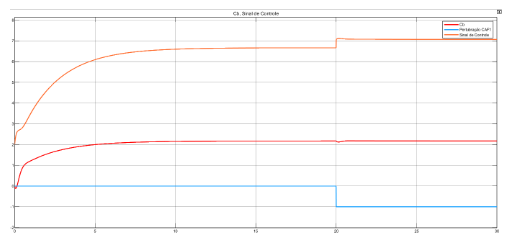
\includegraphics[width=0.8\linewidth]{image14.png}
    \caption{Nova resposta do sistema linear}    
\end{figure}

Analisando o diagrama de polo e zero

Para analisar a resposta do sistema devemos realizar operações com blocos no diagrama de blocos do sistema linear visto abaixo . 

\begin{figure} [H]
    \centering
    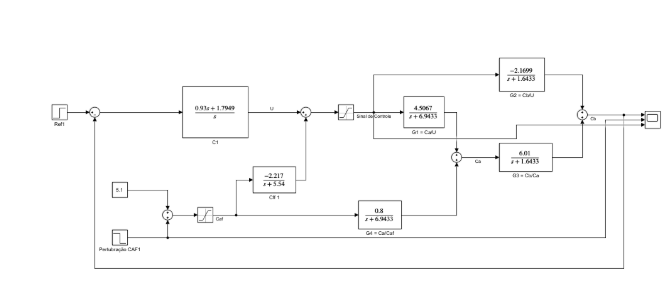
\includegraphics[width=0.8\linewidth]{image15.png}
    \caption{Diagrama de blocos do sistema linear com Cff1}
    
\end{figure}

\begin{align}
C_b &= G_2 \cdot U' + G_3 \cdot Ca, \\
C_b &= G_2 (U + C_{ff} \cdot Q) + G_3 (G_1 \cdot U' + G_4 \cdot Q), \\
C_b &= G_2 (C_1 \cdot E + C_{ff} \cdot Q) + G_3 (G_1 (U + C_{ff} \cdot Q) + G_4 \cdot Q), \\
C_b &= G_2 (C_1 (R - C_b) + C_{ff} \cdot Q) + G_3 (G_1 (C_1 \cdot E + C_{ff} \cdot Q) + G_4 \cdot Q), \\
C_b &= G_2 (C_1 (R - C_b) + C_{ff} \cdot Q) + G_3 (G_1 (C_1 (R - C_b) + C_{ff} \cdot Q) + G_4 \cdot Q), \\
C_b &= \frac{G_2C_1R - G_2C_1C_b + G_2C_{ff}Q + G_3G_1C_1R - G_3G_1C_1C_b + G_3G_1C_{ff}Q}{1 + G_2C_1 + G_3G_1C_1}, \\
C_b &= \frac{(G_2C_1 + G_3G_1C_1)R + (G_2C_{ff} + G_3G_1C_{ff})C_a + (G_3G_4)Q}{1 + G_2C_1 + G_3G_1C_1}.\\
C_b &= \frac{(G_2C_1 + G_3G_1C_1)R}{1 + G_2C_1 + G_3G_1C_1}+\frac{(G_3G_4)Q}{1 + G_2C_1 + G_3G_1C_1}
\end{align}

Onde Q = Ccaf e R = U

Utilizando o seguinte controlador feed-foward:

\begin{align}
C_{ff} = \frac{-2.217}{(s+5.54)} 
\end{align}


Substituindo os valores, obtemos a seguinte função transferência para a perturbação:

\begin{figure} [H]
    \centering
    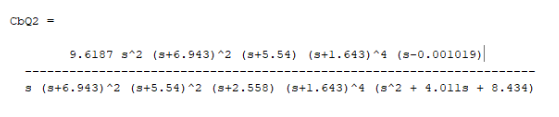
\includegraphics[width=0.8\linewidth]{image16.png}
    \caption{Equação Função C_b}    
\end{figure}

\begin{align}
\frac{C_b}{C_{af}} = \frac{9.6187s^2}{(s+5.54)(s+2.558)(s^2+4.011s+8.434)}
\end{align}

De acordo com a resposta em relação a perturbação obtida, temos o seguinte diagrama de polos e zeros:

\begin{figure}[H]
    \centering
    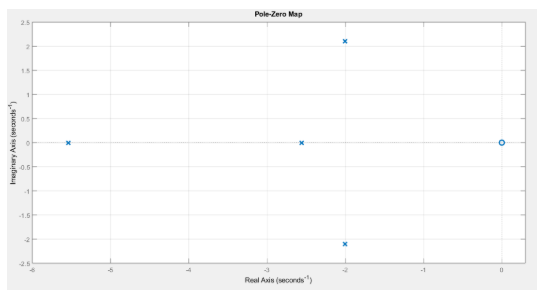
\includegraphics[width=0.8\linewidth]{image17.png}
    \caption{Diagrama de polos e zeros de \( \frac{C_b}{C_{af}} \)}
\end{figure}

Observando o diagrama de polos e zeros da resposta \(C_b\)/\(C_{ff1}\) acima, nota-se a presença de um zero dominante que irá causar sobressinal e aceleramento da resposta.

Utilizando agora o seguinte controlador Feed-Foward:

\begin{align}
C_{ff} = 0.4
\end{align}

Substituindo os valores, obtemos a seguinte função transferência para a perturbação:
\begin{align}
    \frac{C_B}{C_{af}} = \frac{(0.86796s^2 + 6.943 s + 1.643 s + 0.0004607)}{s(s + 6.943s + 2.558s + 1.643s + 4.011s + 8.434)}\\
\frac{C_B}{C_{af}} = \frac{0.86796s^2}{ (s+ 2.558)  (s^2+ 4.011s + 8.434)}
\end{align}


De acordo com a resposta em relação a perturbação obtida, temos o seguinte diagrama de polos e zeros:

\begin{figure} [H]
    \centering
    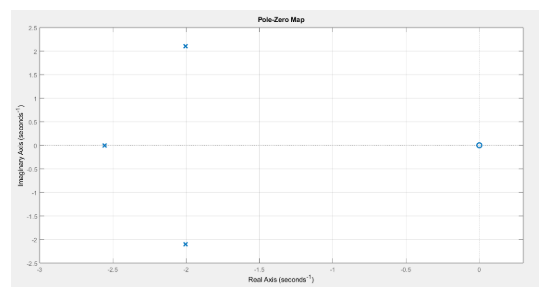
\includegraphics[width=0.8\linewidth]{image18.png}
    \caption{Diagrama de polos de C_b/C_{af}}
    
\end{figure}

Do mesma forma que o anterior, nota-se novamente a presença do zero dominante.
Contudo, com esse controlador nós obtemos um número menor de polos, oque irá deixar a resposta mais rápida. 

Para comparar iremos plotar as respostas de ambos controladores: 

\begin{figure} [H]
    \centering
    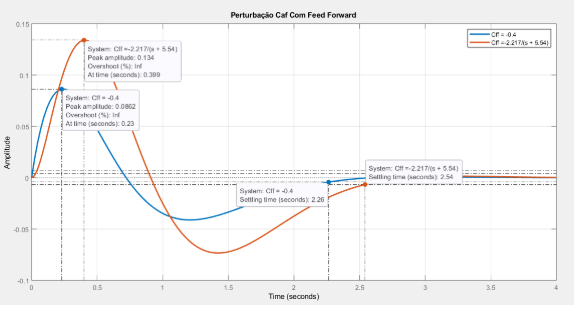
\includegraphics[width=0.8\linewidth]{image19.png}
    \caption{Resposta do sistema com os 2 controladores}
    
\end{figure}

Como analisado anteriormente, vemos que a resposta com a segunda aproximação para o Cff foi mais rápida pois apresenta um polo a menos. Nota-se também que o máximo pico da segunda aproximação apresentou um menor valor para o máximo pico.

Agora para o controle Feed-Foward de \(C_a\) temos o seguinte:

\begin{figure} [H]
    \centering
    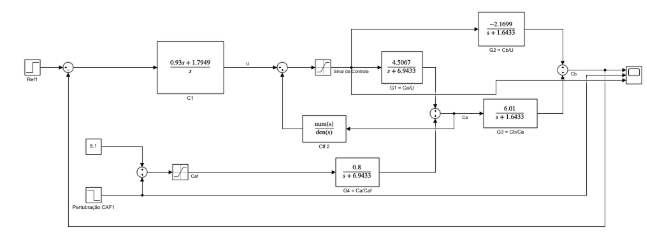
\includegraphics[width=0.8\linewidth]{image20.png}
    \caption{Diagrama de blocos do sistema linear com Cff2}
    
\end{figure}

\begin{align}
(s + 1.6433)C_b = 6.01C_a - 2.1699U\\
\frac{C_a}{C_b} = \frac{6.01}{s + 1.6433} = C_{ff2}\\
C_{ff2} = \frac{C_{q2}}{G} = \frac{\frac{6.01}{(s+1.64)}}{\frac{-2.17(s-5.54)}{(s+6.94)(s+1.64)}}\\
\frac{C_{q2}}{G} = \frac{2.77(s+6.94)}{s-5.54}= \frac{-2.77(s+6.94)}{-s+5.54} 
\end{align}

Mais uma vez temos um polo no semiplano direito, podemos fazer as mesmas aproximações anteriores, dessa forma temos:

Aproximação trocando o polo:
\begin{align}
C_{ff2} = \frac{-2.77(s+6.94)}{-s+5.54} 
\end{align}

Aproximação pelo ganho:

\begin{align}
C_{ff2} =\frac{-2.77(0+6.94)}{0-5.54} = \frac{2.77*6.94}{-5.54} = -3.47
\end{align}


Analisando o diagrama de polo e zero e resposta do sistemas:

Para analisar a resposta do sistema devemos realizar operações com blocos no diagrama de blocos do sistema linear visto abaixo . 

\begin{figure} [H]
    \centering
    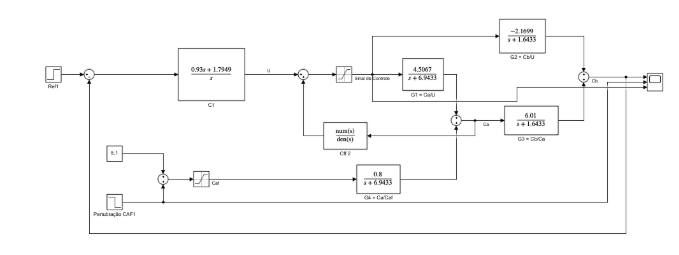
\includegraphics[width=0.8\linewidth]{image21.png}
    \caption{Diagrama de blocos do sistema linear com Cff2}
    
\end{figure}

\begin{align}
C_b &= G_2 \cdot U' + G_3 \cdot C_a, \\
C_b &= G_2 (C_1 (R - C_b) + C_{ff} \cdot C_a) + G_3 (G_1 (C_1 (R - C_b) + C_{ff} \cdot C_a) + G_4 \cdot C_{af}), \\
C_b &= G_2 C_1 R - G_2 C_1 C_b + G_2 C_{ff} C_a + G_3 G_1 C_1 R - G_3 G_1 C_1 C_b + G_3 G_1 C_{ff} C_a + G_3 G_4 C_{af}, \\
C_b &= \frac{G_2 C_1 R + G_3 G_1 C_1 R + (G_2 C_{ff} + G_3 G_1 C_{ff}) C_a + G_3 G_4 C_{af}}{1 + G_2 C_1 + G_3 G_1 C_1}, \\
C_b &= \frac{(G_2 C_1 + G_3 G_1 C_1) R + (G_2 C_{ff} + G_3 C_1 C_{ff}) C_a + (G_3 G_4)C_{af}}{1 + G_2 C_1 + G_3 G_1 C_1 C_{af}}
\end{align}


Utilizando a primeira aproximação para \(C_{ff2}\)

\begin{align}
C_{ff2} = \frac{-2.77(s+6.94)}{s+5.54}
\end{align}

Obtemos a seguinte resposta para a perturbação:

\begin{align}
\frac{C_a}{C_b} = \frac{4.816s}{(s+2.552)(s^2+4.016s+8.84)}
\end{align}

Utilizando a segunda aproximação para \(C_{ff2}\)
\begin{align}
C_{ff2} = -3.47
\end{align}

Obtemos a seguinte resposta para a perturbação:
\begin{align}
\frac{C_b}{C_a} = \frac{4.816s}{(s+2.552)(s^2+4.016s+8.484)}
\end{align}

Que é muito próxima à anterior.

De acordo com a resposta em relação a perturbação obtida, temos o seguinte diagrama de polos e zeros:

\begin{figure} [H]
    \centering
    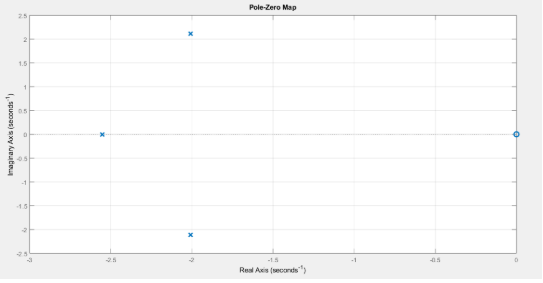
\includegraphics[width=0.8\linewidth]{image22.png}
    \caption{Diagrama de polos e zeros de C_b/Ca}
    
\end{figure}

Visto o diagrama de polos e zeros acima, nota-se a presença de zero dominante, que causará na resposta do sistema um sobressinal, além de polos complexos que irão causar oscilação

Plotando resposta em relação a perturbação obtemos o seguinte gráfico:

\begin{figure} [H]
    \centering
    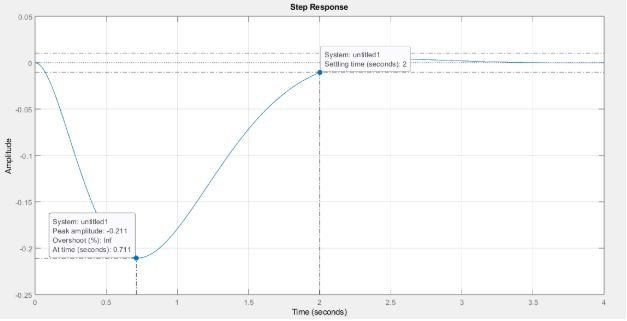
\includegraphics[width=0.8\linewidth]{image23.png}
    \caption{Resposta do sistema com o novo controlador Feed-Forward Cff2}
    
\end{figure}

De acordo com o gráfico da resposta acima, nota-se que a existência do sobressinal causado pelo zero dominante, assim como também oscilação advinda dos polos complexos.


b) Implemente em MATLAB (no tempo discreto) a solução escolhida, definindo adequadamente \(T_s\) e supondo um sustentador de ordem zero no sistema AD/DA.

Com o desenvolvimento da questão anterior, percebemos que utilizando o Feedforward na concentração de \(C_a\) é possível melhorar o tempo de assentamento da perturbação, mas o Feedforward de \(C_{af}\) resulta em um pico máximo de perturbação menor.


Além disso, percebemos que, utilizando apenas o ganho estático no Feedforward de \(C_{af}\), foi possível obter uma resposta mais satisfatória, pois o tempo de assentamento foi menor e o pico máximo da oscilação também foi reduzido. Assim, concluímos que o melhor método a ser utilizado é a aproximação pelo ganho estático utilizando Feedforward em \(C_{af}\).


De acordo com as analises dos gráficos acima obtemos o seguinte tempo de amostragem:
\[
T_s \leq \frac{t_{5\%}}{20} = \frac{1.5}{20} = 0.07min
\]

Iremos discretizar agora através do método Forward onde:

\[
s = \frac{z-1}{T_s} 
\]

Temos que o nosso controlador é:

\[
C_(s) = \frac{0.93*(s+1.93)}{s} = \frac{0.93s+1.7949}{s} =
\frac{0.93\frac{z-1}{T_s}+1.7949}{\frac{z-1}{T_s}}\]
\[
C_z = \frac{0.93z-1+17949T_s}{z-1} = \frac{0.93z + 1.7949T - 0.93}{z-1}
\frac{U}{E} = \frac{0.93z + 1.7949T - 0.93}{z-1}
\]

Obtendo as equações de diferenças do controlador:

\[
U(z - 1) = E(0.93z + (1.7949T_s - 0.93))
\]
\[
U[k + 1] - U[k] = 0.93E[k + 1] + (1.7949T_s - 0.93)E(k)
\]
\[
U[k] = U[k - 1] + 0.93E[k] + (1.7949T_s - 0.93)E[k - 1]
\]

Como \(C_{ff}\) = - 0.4, não precisa ser discretizado, pois é só um ganho agora, utilizando Matlab, podemos criar o seguinte código:

% Configuração do ambiente listings para código MATLAB
\lstset{
    language=Matlab,
    basicstyle=\ttfamily\small,
    numbers=left,
    numberstyle=\tiny,
    stepnumber=1,
    numbersep=5pt,
    backgroundcolor=\color{white},
    showspaces=false,
    showstringspaces=false,
    showtabs=false,
    frame=single,
    rulecolor=\color{black},
    tabsize=2,
    captionpos=b,
    breaklines=true,
    breakatwhitespace=true,
    title=\lstname,
    keywordstyle=\color{blue},
    commentstyle=\color{green!50!black},
    identifierstyle=\color{black},
    stringstyle=\color{mauve},
    escapeinside={(*@}{@*)}, % Para adicionar LaTeX dentro do código
}


\begin{lstlisting}[caption={Código MATLAB para simulação de controle}]
close all
clear
clc

Ts = 0.07;

% -------------------- Sinal de Referencia ---------------------------
t_final = 50; % tempo total de simulacao
t = 0:Ts:t_final; % vetor de tempo
t_rampa = 8; % duracao da rampa
rampa_slope = 2 / t_rampa; % inclinacao da rampa
rampa_offset = 0; % valor inicial da rampa
rampa_final_value = 2.17; % valor final apos a rampa
R = rampa_slope .* (t - rampa_offset) .* (t <= t_rampa) + rampa_final_value .* (t > t_rampa);
R(t >= 25) = 2.17; % mudanca de valor a partir de T = 20

plot(t, R, 'LineWidth', 2, 'Color', 'red');
hold on;

% --------------------- Perturbacao Caf ------------------------------

caf = 5.1 * ones(size(t)); % vetor inicialmente com valor 5.1 para todos os tempos
qcaf = 0 * ones(size(t));

qcaf(t >= 30) = -0.5; % mudanca de valor a partir do tempo t = 40

% Inicializacao das variaveis do processo
k1 = 6.01;
k2 = 0.8433;
k3 = 0.1123;

nit = round(t_final / Ts); % numero de iteracoes do laco de controle

Ca = zeros(1, nit + 1);
C_b = zeros(1, nit + 1);
U = zeros(1, nit + 1);

rfant = 0;
eant = 0; % como o sistema e ligado desde o inicio, todos sao zero
u1ant = 0;
Cff = -0.4;

caf = caf + qcaf;

% Laço de Controle
for k = 2:nit + 1
    % sistema de controle
    y = C_b(k - 1);
    %rf = 0.1533016*R(k-1) + 0.8466984*rfant;
    e = R(k - 1) - y;
    u1 = u1ant + 0.93 * e + (1.7949 * Ts - 0.93) * eant;
    u2 = (Cff * caf(k - 1));

    u1ant = u1;
    eant = e;

    u = u1 + u2;

    % saturacao do sinal de controle
    if u >= 10
        u = 10;
    end

    if u <= 0
        u = 0;
    end

    U(k - 1) = u; % para o plot do sinal de controle

    % atualizacao das variaveis de controle
    %rfant = rf;

    % simulacao do processo com modelo nao linear
    Ca(k) = (-k1 * Ca(k - 1) - u * Ca(k - 1) - k3 * ((Ca(k - 1))^2) + caf(k1) * u) * Ts + Ca(k - 1);
    C_b(k) = (k1 * Ca(k - 1) - k2 * C_b(k - 1) - C_b(k - 1) * u) * Ts + C_b(k - 1);

end

% plot sinais de referencia, ca e C_b
plot(t, C_b, 'LineWidth', 2, 'Color', 'blue');
plot(t, Ca, 'LineWidth', 2, 'Color', 'green');
grid on;
legend('Referência', 'C_b', 'Ca');
xlabel('Tempo [min]');
ylabel('Concentração [mol/l]');
title('Concentração de C_b e Ca com Referência Para C_b e Perturbação em Caf');

% plot principais sinais
figure();
plot(t, U, 'LineWidth', 2, 'Color', 'blue');
hold on
plot(t, caf, 'LineWidth', 2, 'Color', 'red');
plot(t, C_b, 'LineWidth', 2, 'Color', 'black');
plot(t, R, 'LineWidth', 2, 'Color', 'green', 'LineStyle', '--');

grid on;
legend('Sinal de Controle', 'Caf', 'C_b', 'Referência');
xlabel('Tempo [min]');
ylabel('Amplitude');


legend('Sinal de Controle u', 'Perturbação de Caf', 'Concentração de \(C_b\)', 'Referência');
grid on;
title('Principais Sinais');
xlabel('Tempo [min]');
ylabel('Amplitude');


\end{lstlisting}




Isso nos gera os seguintes gráficos:

\begin{figure} [H]
    \centering
    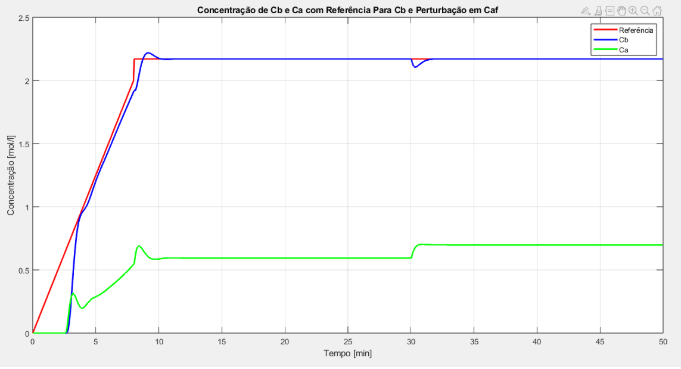
\includegraphics[width=0.8\linewidth]{image4.png}
    \caption{Concentração de \(C_b\) e Ca com variação de \(C_{af}\)}
    
\end{figure}

\begin{figure} [H]
    \centering
    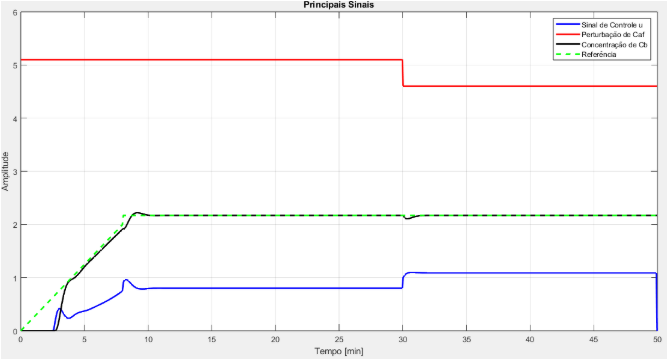
\includegraphics[width=0.8\linewidth]{image5.png}
    \caption{Principais Sinais}
    
\end{figure}

Como pode ser observado nos gráficos acima, a perturbação é rejeitada de maneira aceitável, pois com o controlador Feed-Forward a perturbação tem efeito sobre a concentração de \(C_b\) um pico máximo muito pequeno e com duração de aproximadamente 
1,2 minutos.

\begin{figure} [H]
    \centering
    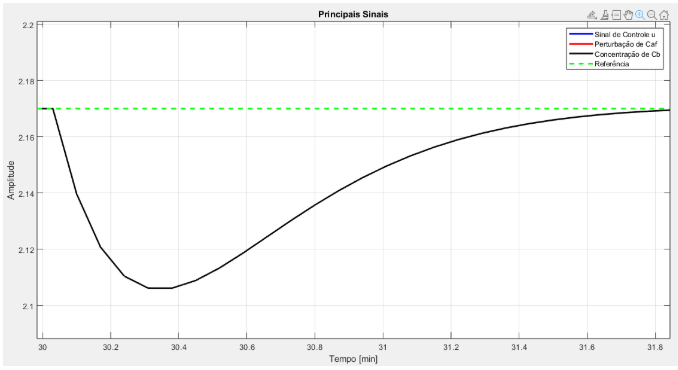
\includegraphics[width=0.8\linewidth]{image6.png}
    \caption{Perturbação na concentração de \(C_b\) causado pela variação de \(C_{af}\)}
   \end{figure}

\newpage
\subsection{Simulação Não Linear}

Simule agora o sistema não linear controlado em MF com a sua proposta de controle. 
Utilize um cenário onde o sistema é levado até o ponto de operação em modo 
automático com uma rampa de aproximação (defina uma rampa de referência 
adequada). Aplique perturbações e simule ruídos de medição para obter um cenário 
próximo da realidade. Analise os sinais, compare os resultados com os da parte 1 e 
discuta.

Utilizando o que foi montado na questão anterior e adicionando ruídos têm-se o seguinte diagrama de blocos e o seguinte gráfico. Para simular de maneira mais próxima à realidade, utilizamos o controlador discreto e o sistema não linear continuo. Adicionamos blocos de ruido nas leituras dos sensores de concentração de \(C_b\) e também na concentração de \(C_{af}\)

\begin{figure} [H]
    \centering
    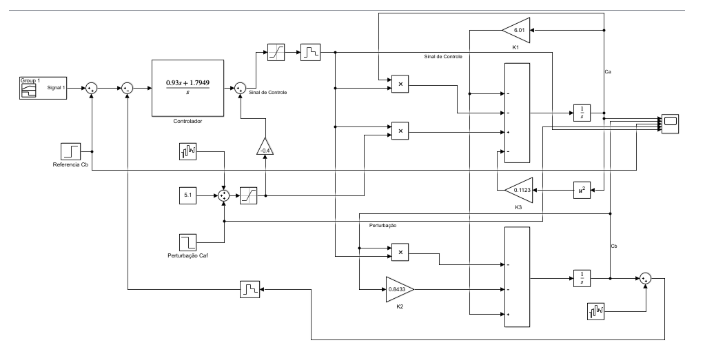
\includegraphics[width=0.8\linewidth]{image1.png}
    \caption{Diagrama de polos do sistema com controlador Cff1}   
\end{figure}

Iniciando a simulação, obtivemos a seguinte resposta:

\begin{figure} [H]
    \centering
    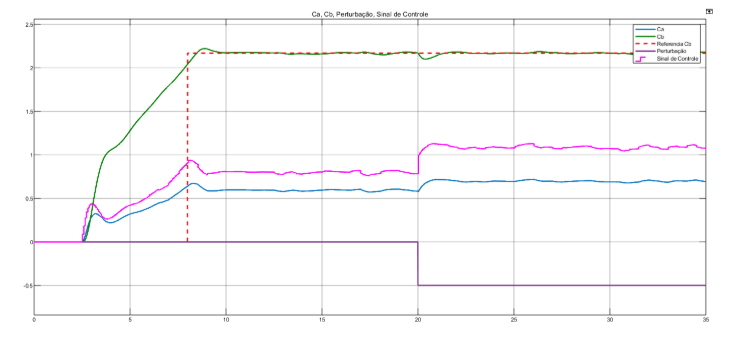
\includegraphics[width=0.8\linewidth]{image2.png}
    \caption{Resposta do sistema com controlador Cff1 à perturbação}
\end{figure}

Como podemos observar, o sistema rejeitou de maneira muito satisfatória a perturbação inserida em \(C_{af}\) , praticamente não foi possível observar mudanças na concentração de \(C_b\).

Com relação à parte 1 do trabalho, podemos ver que o uso do Feed-Forward garantiu uma resposta muito melhor da perturbação.

\begin{figure} [H]
    \centering
    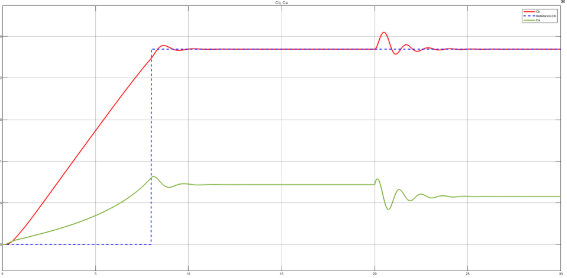
\includegraphics[width=0.8\linewidth]{image3.png}
    \caption{Resposta do sistema da parte 1 sem o controlador Cff1}
\end{figure}

Dessa forma, concluímos que mesmo que seja mais trabalhoso e computacionalmente mais pesado, o Feed-Forward nos gera uma resposta bem melhor às variações da Perturbação, que mal foram visíveis, enquanto que sem o Feed-Forward, obtivemos
oscilações. 

Outro ponto a ser levado em consideração foi que o uso de Lugar da Raízes gerou menos oscilações na resposta, enquanto que o controlador obtido na parte 1, as oscilações
ocorriam com frequência.
  
\end{document}